
\documentclass{beamer}
\usepackage{bm}
\usetheme{Madrid}
\title{The BFGS Optimization Algorithm}
\author{Pratham Lalwani}
\institute{UC Merced}
\date{\today}

\newcommand{\incfig}[1]{%
		\def\svgwidth{\columnwidth}
		\import{./figs/}{#1.png}
	}
\begin{document}

\frame{\titlepage}

\begin{frame}{Outline}
	\tableofcontents
\end{frame}

%------------------------------------------------
\section{Background}
\begin{frame}{Problem Setup}
	\begin{itemize}
		\item Given $f:\mathbb{R}^n \to \mathbb{R}$, say we are interested is minimizing the function, which is,
		      \[
			      \min_{\bm x\in \mathbb{R}^n} f(\bm x)
			      .\]
		\item From calculus, $\nabla f(\bm x) = \bm 0$ and solve analytically if it can be done.
		\item This problem arises everywhere especially nowadays with Machine Learning where $f(\bm x)$ is usually a cost function we are trying to minimize.
	\end{itemize}
\end{frame}

\begin{frame}{Gradient Descent and Its Limitations}
	\begin{itemize}
		With no way to compute a analytic solution one might turn a simple algorithm like Gradient Descent.
		\item The next iterate is given by : $\bm x_{k+1} = \bm x_k - \gamma \nabla f(\bm x_k)$, where $\gamma$ is a fixed constant called step size or learning rate.
		\item Pros: simple, easy to implement and not computationally expensive (per step)
		\item Cons: slow convergence, sensitivity to step size.
	\end{itemize}
\end{frame}

\begin{frame}[t]
	\frametitle{Gradient Descent}
	\begin{figure}[htpb]
		\centering
		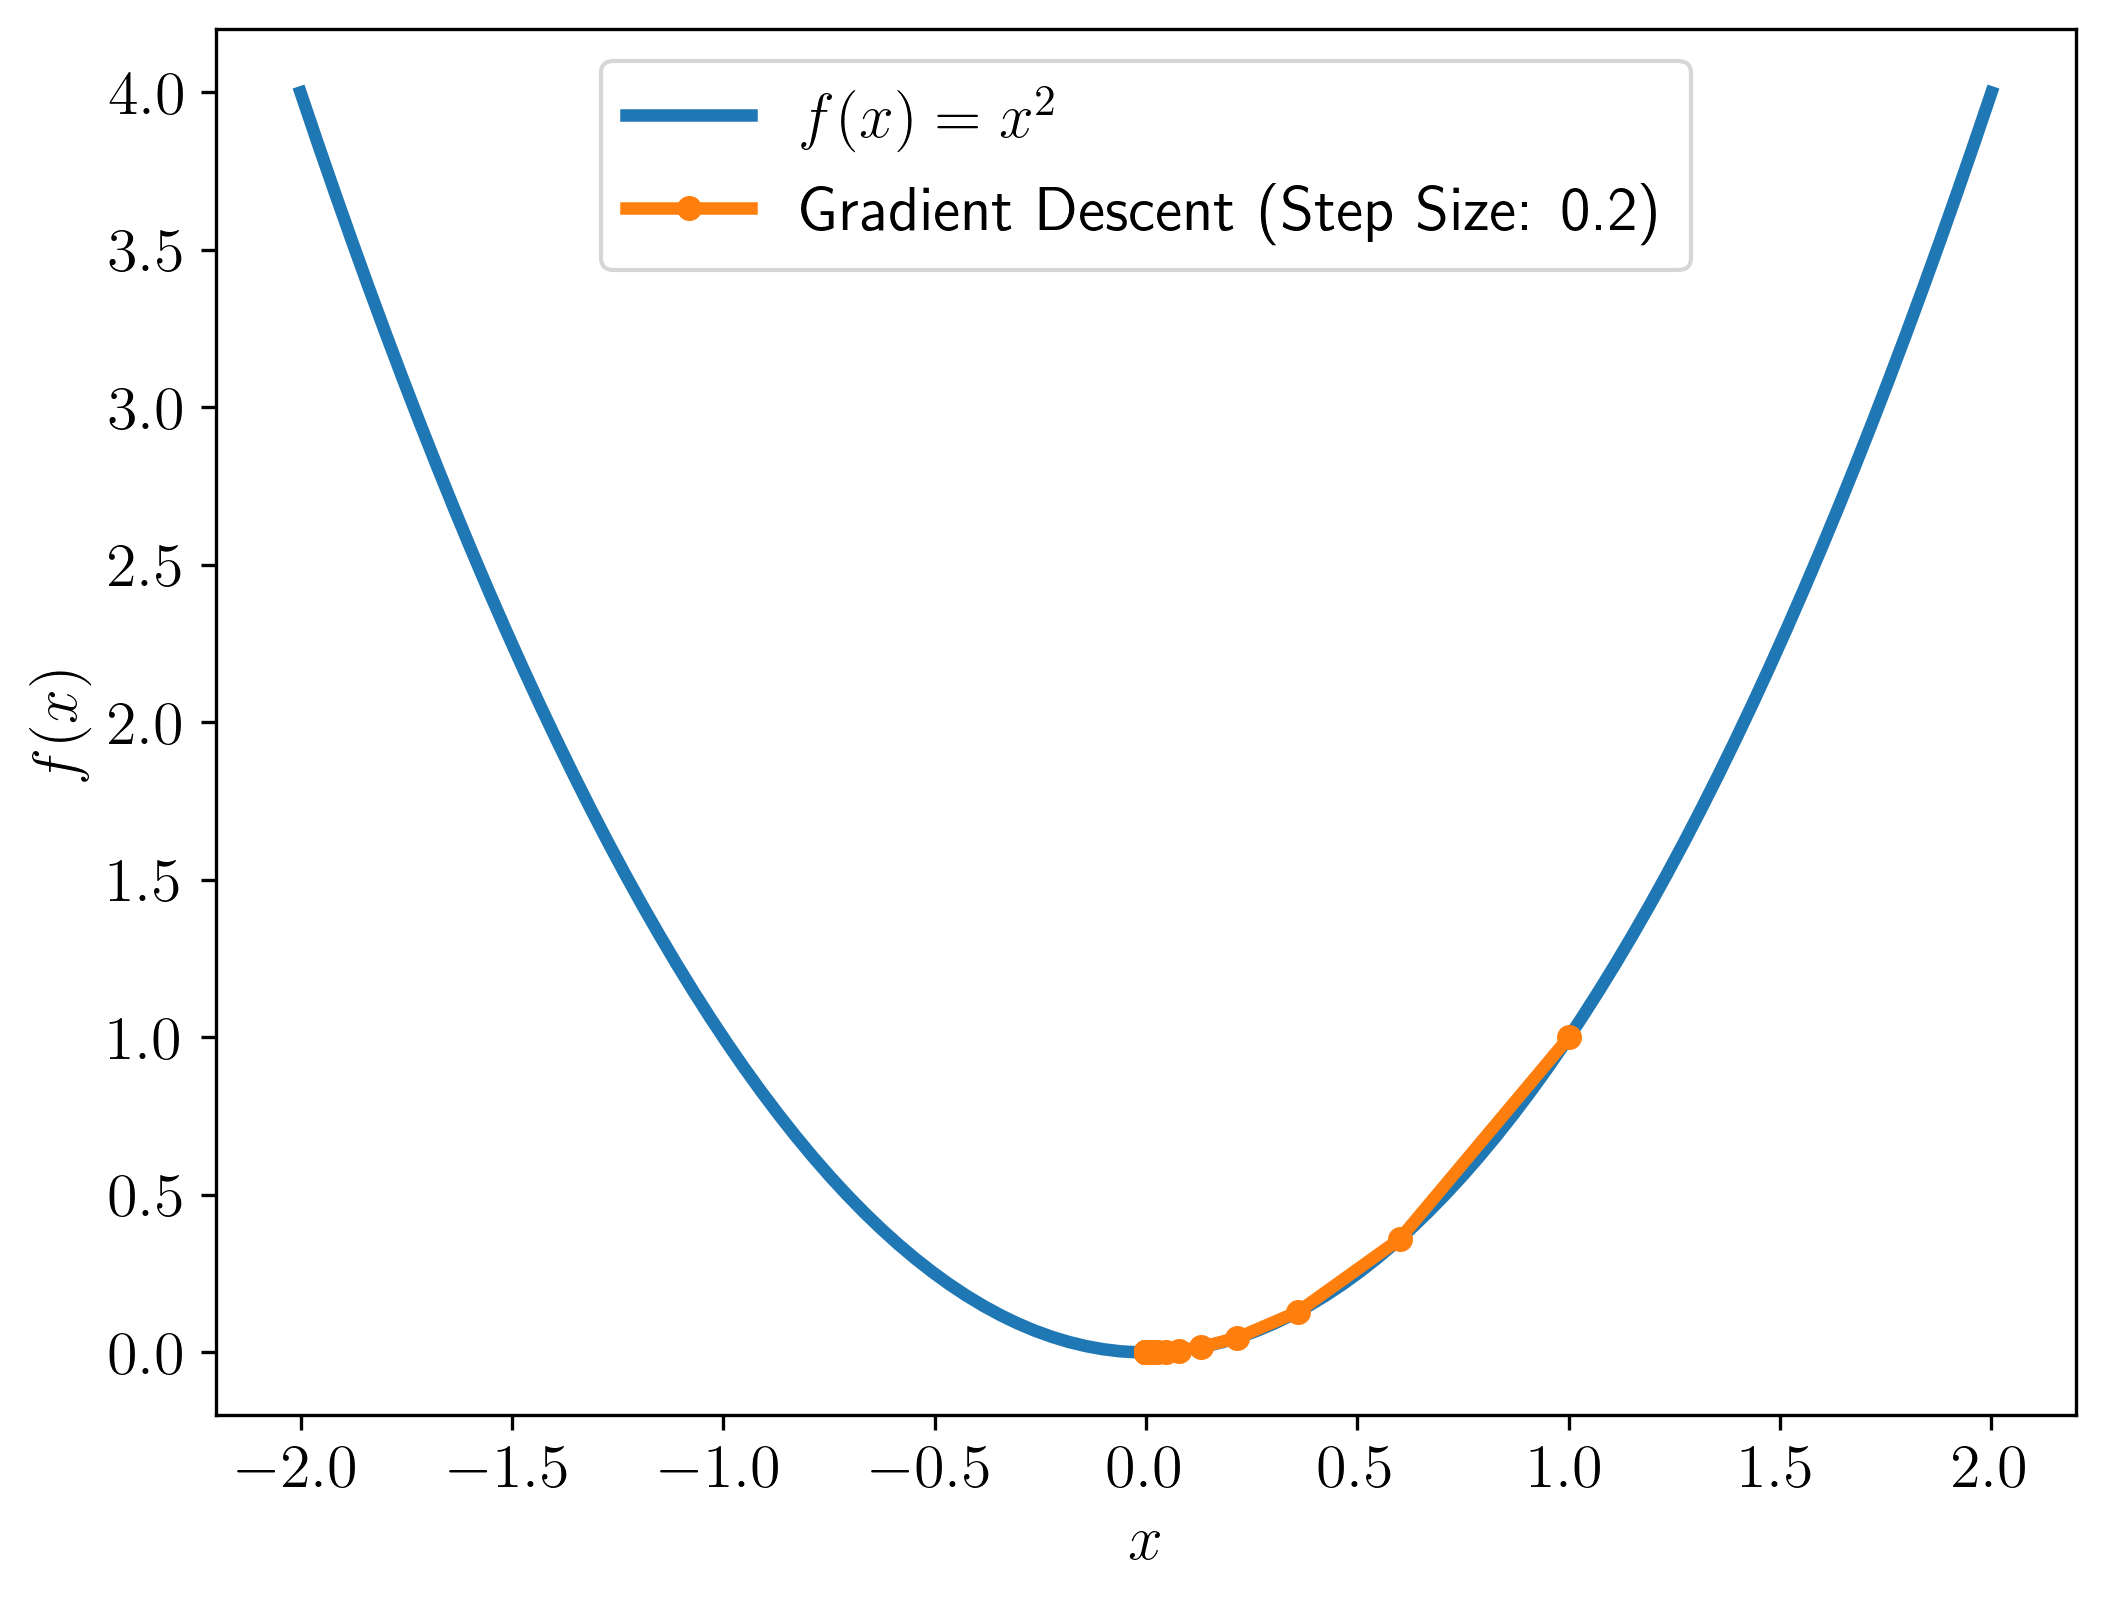
\includegraphics[width=0.7\textwidth]{./figs/gradient_descent_low_learning_rate}
		\caption{Gradient Descent on $x^2$}
		\label{fig:}
	\end{figure}
\end{frame}
\begin{frame}[t]
	\frametitle{Gradient Descent}
	\begin{figure}[htpb]
		\centering
		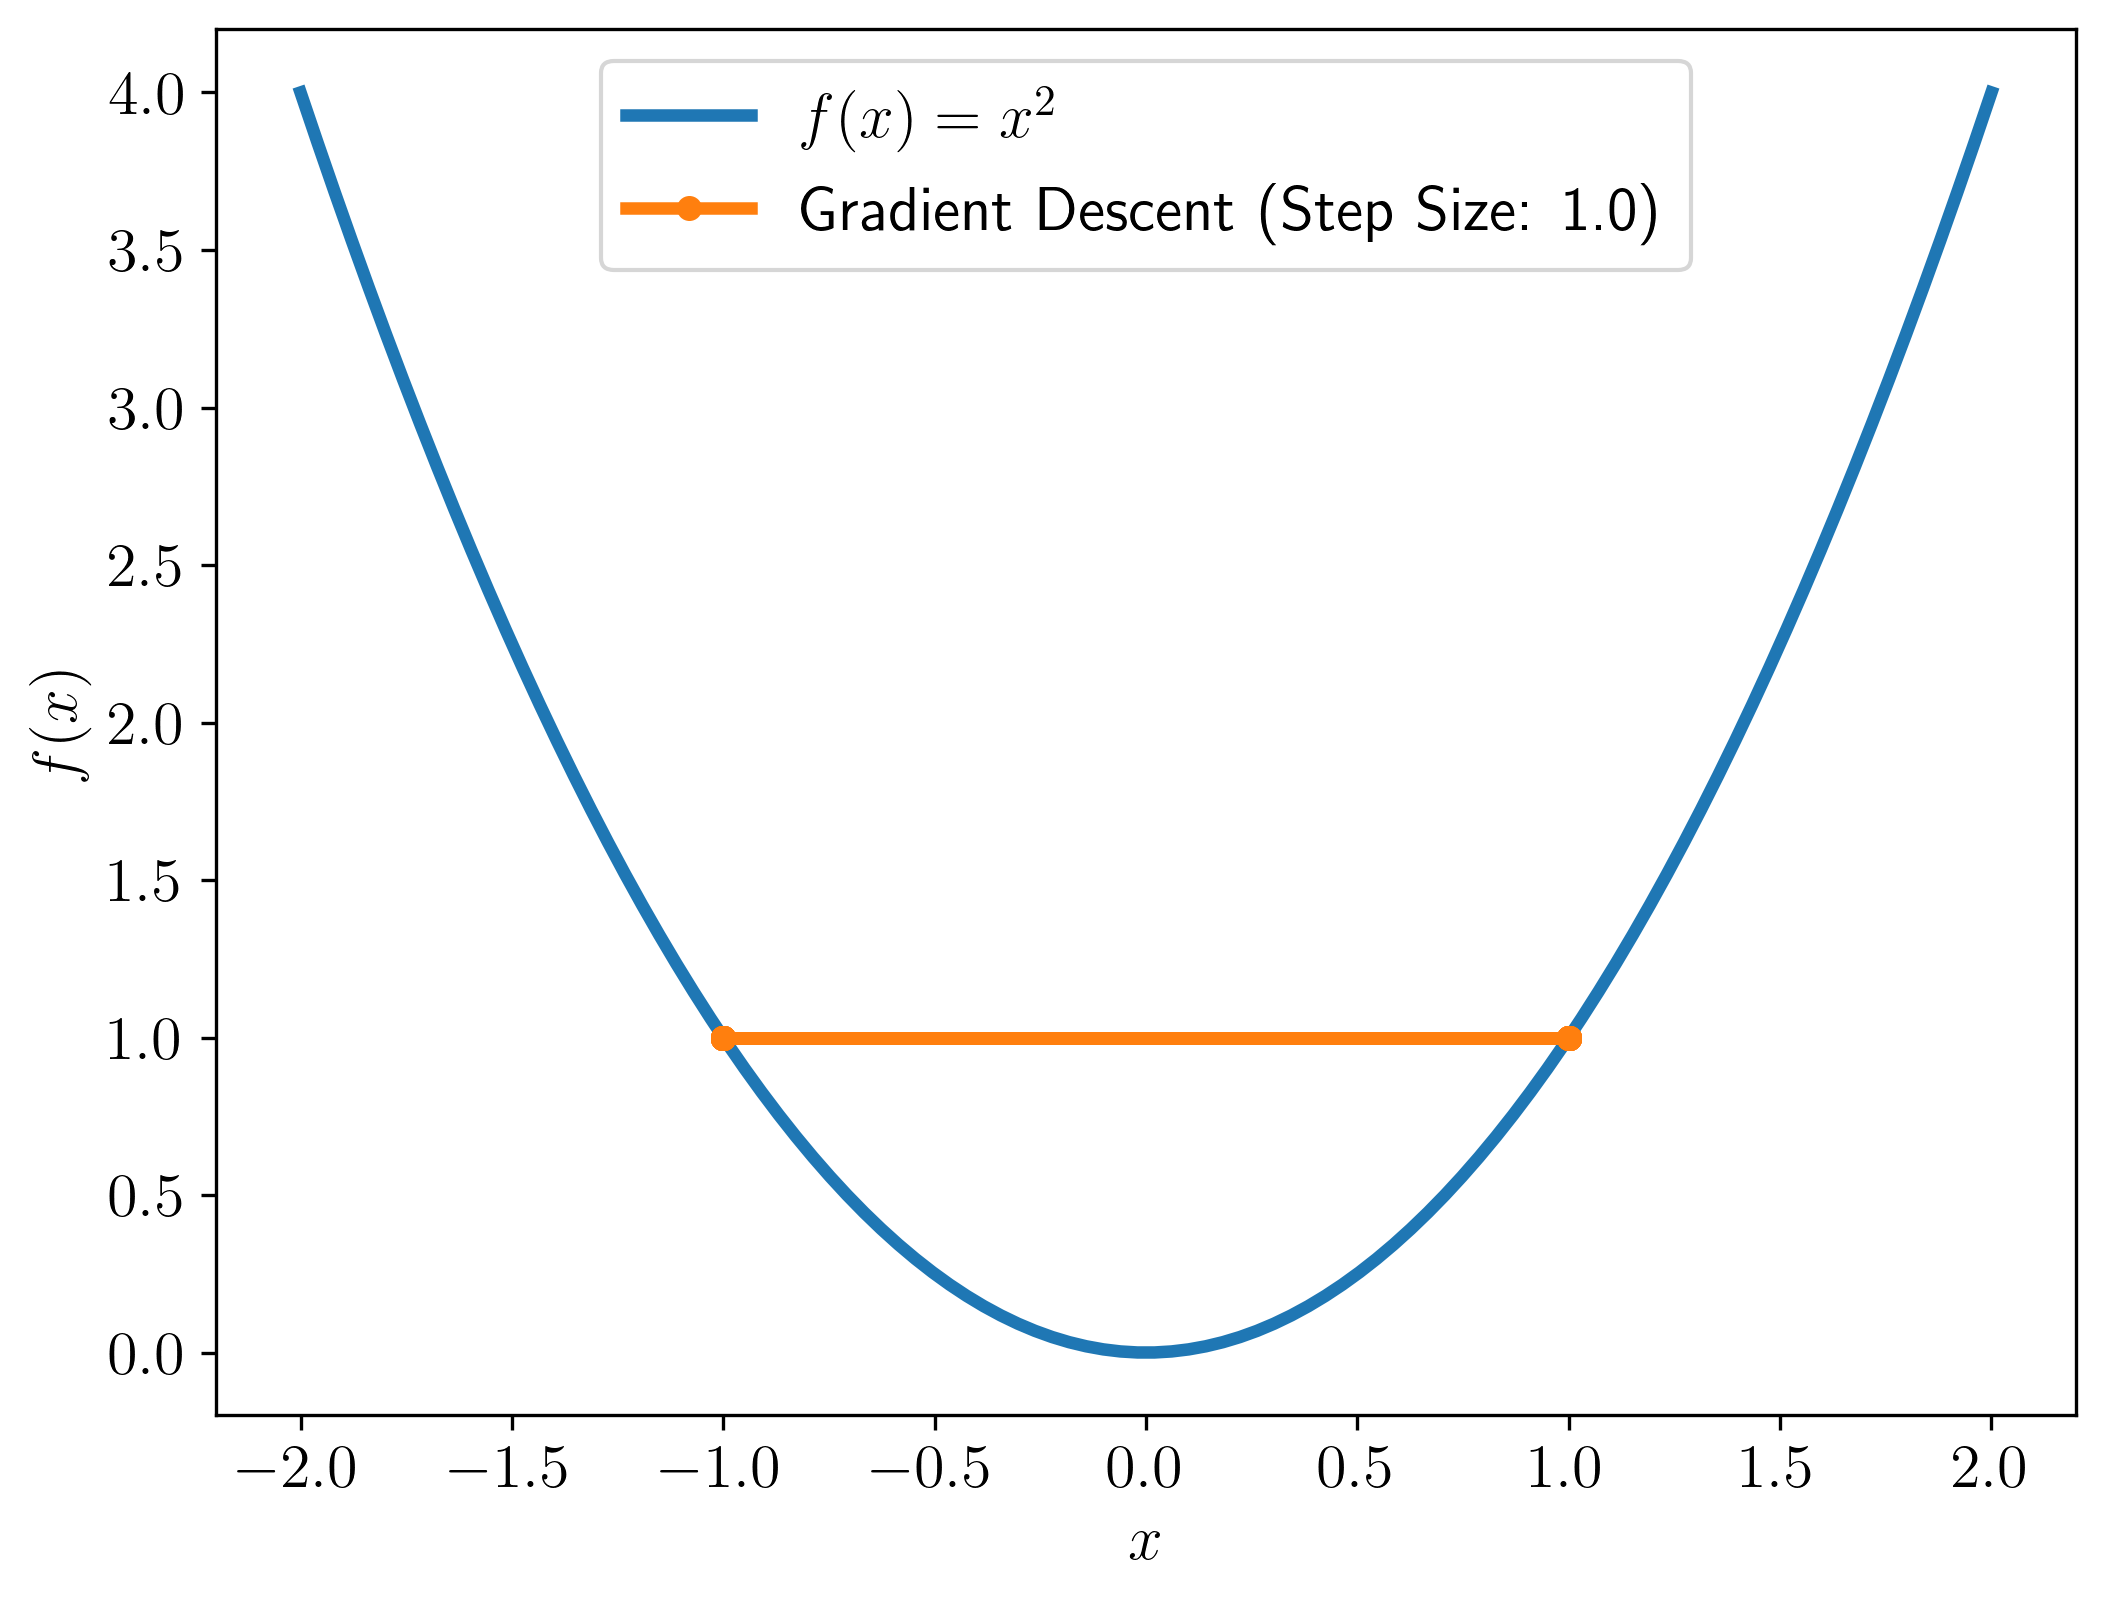
\includegraphics[width=0.7\textwidth]{./figs/gradient_descent_high_learning_rate}
		\caption{Gradient Descent on $x^2$}
		\label{fig:}
	\end{figure}
\end{frame}
%------------------------------------------------
\begin{frame}[t]
	\frametitle{But wait a minute}
	Instead of having a fixed Learning Rate what if we have a adaptive learning rate, which is "greedy".
	If we have,
	\[
		\bm x_{k+1} = \bm x_{k} - \alpha_k \nabla f(\bm x)
		.\]\pause
	We define,
	\[
		\phi(\alpha) := f(\bm x_k-\alpha \nabla f(\bm x))
		.\]
\end{frame}
%------------------------------------------------
\section{Quasi-Newton Methods}
\begin{frame}{History of Quasi-Newton Algorithms}
	\begin{itemize}
		\item Aim: approximate Hessian without second derivatives
		\item Early methods: Davidon–Fletcher–Powell (DFP)
		\item Development of symmetric rank-one (SR1), BFGS
	\end{itemize}
\end{frame}

%------------------------------------------------
\section{BFGS Algorithm}
\begin{frame}{The BFGS Algorithm}
	\begin{itemize}
		\item Builds positive-definite Hessian approximation $B_k$
		\item Update: $B_{k+1} = B_k + \frac{y_k y_k^T}{y_k^T s_k} - \frac{B_k s_k s_k^T B_k}{s_k^T B_k s_k}$
		\item Search direction: $p_k = -B_k^{-1} \nabla f(x_k)$
		\item Widely used: stable and fast convergence
	\end{itemize}
\end{frame}

%------------------------------------------------
\section{Rosenbrock Example}
\begin{frame}{Rosenbrock Example}
	\begin{itemize}
		\item Test function: $f(x,y) = (a - x)^2 + b(y - x^2)^2$
		\item Typical parameters: $a=1, b=100$
		\item Illustrates curved valley and optimization challenge
	\end{itemize}
\end{frame}

\begin{frame}{Rosenbrock Example Results}
	\begin{figure}
		\centering
		% Include plot: \includegraphics[width=0.6\textwidth]{rosenbrock_bfgs.png}
		\caption{BFGS optimization path on Rosenbrock function}
	\end{figure}
\end{frame}

%------------------------------------------------
\section{Results}
\begin{frame}{Results}
	\begin{itemize}
		\item Converges in fewer iterations compared to gradient descent
		\item Good performance on moderate-scale problems
		\item Memory cost: $O(n^2)$ storage for Hessian approximation
	\end{itemize}
\end{frame}

%------------------------------------------------
\section{Convergence}
\begin{frame}{Convergence of BFGS}
	\begin{itemize}
		\item Locally superlinear convergence under standard assumptions
		\item Requires line search satisfying Wolfe conditions
		\item Practical performance often close to Newton's method
	\end{itemize}
\end{frame}

%------------------------------------------------
\section{Line Search}
\begin{frame}{Line Search}
	\begin{itemize}
		\item Determines step length $\alpha_k$ along direction $p_k$
		\item Common strategies: backtracking, Wolfe conditions
		\item Ensures sufficient decrease and curvature conditions
	\end{itemize}
\end{frame}

\begin{frame}{Demonstration of Line Search}
	\begin{figure}
		\centering
		% Include plot: \includegraphics[width=0.6\textwidth]{line_search_demo.png}
		\caption{Illustration of backtracking line search}
	\end{figure}
\end{frame}

%------------------------------------------------
\section{Conclusion}
\begin{frame}{Conclusion}
	\begin{itemize}
		\item BFGS balances efficiency and robustness
		\item Widely used in unconstrained optimization
		\item Extensions: limited-memory L-BFGS for large-scale problems
	\end{itemize}
\end{frame}

\end{document}

